\documentclass {article}
\usepackage{enumitem}
\usepackage{listings}
\usepackage{color}
\usepackage{float}
\usepackage{mathtools}
\usepackage{graphicx}
\graphicspath{ {images/} }

\definecolor{mGray}{rgb}{0.39, 0.39, 0.39}
\definecolor{mBlue}{rgb}{0.04, 0.36, 0.67}
\renewcommand*\rmdefault{cmr}

\lstset{ %set options for lstlisting = codesnippets
	basicstyle=\small\ttfamily,
	commentstyle= \small\ttfamily\color{mGray},
	keywordstyle= \color{mBlue},
	numberstyle= \footnotesize\ttfamily\color{mGray},
	breaklines=true,
	captionpos=b,
	numbers=left,
	tabsize=2,
	keepspaces=true,
	showspaces=false,
	showstringspaces=false
}

\setlength{\parindent}{0em}
\setlength{\parskip}{1em}

\title{A comparison between functional and object oriented programming approaches in JavaScript}
\date{\today}
\author{
Kim Svensson Sand \and Tord Eliasson
}

\begin{document}
\maketitle
\pagenumbering{gobble}
\newpage
\tableofcontents
\newpage
\pagenumbering{arabic}
\section*{Abstract}
\subsection*{Keywords}
\listoffigures
\listoftables
\section*{Abbreviations}
\begin{itemize}[leftmargin=*]
\item [ ] ES6 = ECMAScript 2015
\item [ ] FP = Functional Programming
\item [ ] OOP = Object-Oriented Programming
\end{itemize}
\section{Introduction}
Programming paradigms is a way to classify a certain way of programming \cite{programming-paradigms}. Each paradigm has its own set of rules for how the code should be written. Some programming languages make it possible to write code according to one paradigm,  while others make it possible to write according to multiple paradigms. 

In the 1950's and 60's multiple high-level languages were developed, that today's programming languages are based upon \cite{gabmar}. These were imperative languages such as Fortran and Algol, functional languages such as Lisp and object-oriented languages such as Simula. Originally Lisp had performance issues and has not been used a lot commercially, but versions of it are still used today. However it is mostly used an academic context. In the 70's C was introduced and quickly established itself thanks to it's ability to access low-level functionality, compact syntax and it's good compiler. In the 80's the object oriented language C++ was developed. It was based on C and and took a lot of inspiration from Simula. Java, that is based on C++ was introduced in the 90's. Since imperative languages gained the upper hand in the 60's and 70's new languages were based on those and continued being the most used. 

Object-oriented or imperative languages are dominating today with languages such as C, C++, Java and C\#. However, functional languages seem to be of interest in the industry again for handling big data and concurrency with languages such as Scala, Erlang or Haskell \cite{drboolean, eriksen, erikarl}. There is a performance difference where functional languages tend to be slower, but there are also positive aspects that could compensate for those, such as memory usage and less code \cite{fogus, alomgi}.  Some are also arguing that a more functional approach will give you more readable code, code that is easier to maintain and easier to test, and that learning it will give you better experience as a programmer \cite{drboolean, meijer}. 

We will compare two programming paradigms, object-oriented programming and functional programming. To compare these we have chosen four different algorithms which we each will implement twice. Once according to the object-oriented paradigm and once according to the functional paradigm. The different algorithms we will implement are tree search algorithms, shellsort algorithm, tower of hanoi algorithm and Dijkstra's algorithm. The comparisons we will make between the algorithms are runtime, memory usage, time of development and lines of code. All algorithms will be written in JavaScript.
\subsection{Research Questions}
\begin{itemize}
\item Will functional versus object-oriented approaches in JavaScript have an impact on performance, such as runtime and memory usage?
\item Can programmers with an object oriented background decrease development time by using practises from functional programming?
\end{itemize}

With the comparison of programming paradigms, the thing that have to be tested is each of the paradigms performance. Because we are writing both paradigms in the same language, we are able to compare just the the paradigms, without having to compare languages and compilers.

We both have studied at BTH, where we learned about programming only according to OOP. Therefore it would be interesting to see how our programming will change, by learning FP. This could give teachers a hum about introducing functional programming to give students a chance to use different paradigms depending on their needs, instead of always using OOP.

We both came from a background of object-oriented programming, therefore 
the question how this will affect our programming will be very interesting. 

Should we write some kind of hypothesis here?

\section{Background and Related work}
Here we will describe the functional programming paradigm, FP, and also the object oriented programming paradigm, OOP. We will also describe JavaScript and it's support for functional and object-oriented methods. The related work described are articles that further explains the positive aspects of functional programming or studies similar to this one.
\subsection{Functional programming}
Functional programming, FP, is a programming paradigm that at its core is based on lambda-calculus \cite{gabmar}. Programs are constructed using functions and by avoiding changing the state. By not modifying the state side effects are avoided. Computation is done by changing the environment, rewriting the functions, rather than changing variables. Multiple functions can be composed into larger and more complex functions, and should be reduced to its simplest state following mathematical rules. The following are concepts used in FP.
\begin{description}
\item [Lazy evaluation] - Lazy evaluation is when a value is not calculated until it is needed \cite{fogus}.
\item [Static type checking] - Pure functional languages usually have static type checking \cite{gabmar}. This means that variables are of a certain type, for example int or char. In such languages it is not allowed to use functions with the wrong types. So if there is for example a function taking an int as parameter it is illegal to call that function with a String as its parameter. In dynamic type checked-languages this would be legal, since variables are not specified as types, and might cause an unexpected error. For example in JavaScript:

\begin{lstlisting}[language=Java]
//JavaScript has dynamic type checking
function double(nr) {
return nr * 2;
}

var word = "string";
double(word); //Will return NaN but still continue running
\end{lstlisting}

\item [ ] A similar program in golang \cite{golang}, that is a statically type checked language:

\begin{lstlisting}[language=Java]
func main() {
  var word string = "string"
  fmt.Printf("%d", double(word)) //Error: cannot use word (type string) as type int in argument to double
}

func double(nr int) int {
  return nr * 2
}
\end{lstlisting}

\item [ ] This will give an error when compiling.
\item[] There are however pure functional languages with dynamic type checking, such as Clean \cite{clean}. There are also languages that are mostly functional with dynamic type checking, such as Common Lisp \cite{commonLisp} or Scheme \cite{scheme} \cite{langTable}.
\item [Side effects] - Side effects are for example changing a variable or any interaction outside the function \cite{drboolean}. This is avoided in functional programming since it may result in incorrect and unexpected behaviour. 
\item [Pure functions] - A pure functions always returns the same result, given the same input, and does not have side effects \cite{drboolean}. See the following example: 

\begin{lstlisting}[language=Java]
var sum = 0;

//Impure
function add(a, b) {
  sum = a + b;
}

//Pure
function add(a, b) {
  var tmp = a + b;
  return tmp;
}
\end{lstlisting}

\item [Higher order functions] - Higher order functions are an important concept in functional programming \cite{fogus}. First class functions mean that functions are treated as values, which means that they can be stored in variables, stored in arrays or created if needed. A higher order function is a first class function that either takes a function as a parameter, returns a function as a result or both. This makes it possible to compose larger and more complex functions.

\begin{lstlisting}[language=Java, breaklines=true]
function add(a, b) {
  return a + b;
}

//Functions can be placed in variables.
var thisFunc = add;

//And also put in other variables.
var sameFunc = thisFunc;
sameFunc(1, 2); //Will give the output 3.

//Functions can also be used as parameters or return values.
function applyFunc(f, a, b) {
  return f(a, b);
}

applyFunc(function(a, b) {
  return a * b;
}, 3, 2); //Will give output of 6

//Returns a function that returns a string
function getStringCreator(category, unit) {
  return function(value) {
    return category + ': ' + value + unit;
  }
}

var weightStringCreator = getStringCreator('Weight', 'kg');
weightStringCreator(5); //Outputs "Weight: 5kg"
\end{lstlisting}

\item [Recursion] - Recursive functions are functions that call themselves and are used as loops \cite{fogus}. It is important in functional programming since it can hide mutable state and also implement laziness. In functional programming recursion is used rather than loops.

\begin{lstlisting}[language=Java]
//Adds all numbers from start to end with a loop
function iterativeAdd(start, end) {
  var sum = 0;
  while(start <= end) {
    sum += start;
    start++;
  }

  return sum;
}

//Adds all numbers from start to end recursively
function recursiveAdd(start, end) {
  if (start == end) {
    return end;
  }
  else {
    return start + recursiveAdd(start + 1, end);
  }
}
iterativeAdd(1, 6); //Outputs 21
recursiveAdd(1, 6); //Also outputs 21
\end{lstlisting}

\item [Currying] - Currying means a function can be called with fewer arguments than it expects and it will return a function that takes the remaining arguments \cite{drboolean}. 

\begin{lstlisting}[language=Java, breaklines=true]
//Returns a new function that takes the remaining argument or the sum of a and b if both are provided.
function addWithCurrying(a, b) {
  if(b) {
    return a + b;
  }
  else {
    return function(b) {
      return a + b;
    }
  }
}

var curryAdd = addWithCurrying(4); 
curryAdd(6); //Outputs 10
addWithCurrying(4, 6); //Also outputs 10
\end{lstlisting}

\item [Immutable data structures] - In functional programming mutations, that are side effects, are avoided \cite{fogus}. Hidden side effects can result in a chains of unpredicted behaviour in large systems. Instead of mutating the data itself a local copy is mutated and returned as a result, as seen in the pure functions example.
\end{description}
\subsection{Object-oriented programming}
Object-oriented programming is a programming paradigm which is built around "objects". These objects may contain data, in form of fields, often referred as attributes and code in form of procedures, often referred to as methods \cite{kindler}.

These objects are created by the programmer to represent something with the help of its attributes and methods. What kind of variables and functions an object should contain is defined in a class, which works like a blueprint for the object. For example, a class can represent an employee. An employee has the attributes assignment and salary. The employee also has a method for doing work. Then the employee has to work somewhere, so we create another object for a company where our employee can work. The company has the attributes income and number of employees. It also has methods to hire employees and fire employees. Since there are more employees who works at this company, we can add more employees by creating new objects of the information in employee class.

By building objects together like this, you can build programs by the object oriented paradigm.  

\begin{description}
\item [Class] - A class is a model for a set of objects, which the object oriented paradigm is built around \cite{gabmar}. The class establishes what the object will contain, for example variables and functions, and signatures and visibility of these. To create a object of any kind, a class must be present. 

\begin{lstlisting}[language=Java]
//Creates a class Animal with the properties name and age and a function for logging the properties to the screen
class Animal {
  constructor (name, age) {
    this.name = name;
    this.age = age;
  }

  logAnimal() {
    console.log('Name: ' + this.name + '\nAge: ' + this.age);
  }
}

var animal = new Animal('Buster', '9');
animal.logAnimal();
//Outputs Name: Buster
//Age: 9
\end{lstlisting}

\item [Object] - An object is a capsule that contains the variables and functions established in the class\cite{}. While objects created from the same class contains the same variables and functions, since the information it contains is handled specifically for every object, the information in the class can vary much. All data and functions can be accessible from outside the object. 

\item [Inheritance] - When an object acquires all properties and functionality of another object \cite{skansholm}. it is called inheritance. This provides code reusability. 

\begin{lstlisting}[language=Java, breaklines=true]
//Based upon the Animal class with an added property race
//The original logAnimal() is overidden so the new property is also logged to the screen.
class Dog extends Animal {
  constructor(name, age, race) {
    super(name, age);
    this.race = race;
  }

  logAnimal() {
    super.logAnimal();
    console.log('Race: ' + this.race);
  }
}

var dog = new Dog('Buster', '9', 'Shitzu');
dog.logAnimal();
//Outputs Name: Buster
//Age: 9
//Race: Shitzu
\end{lstlisting}

\item [Encapsulation] - Encapsulation can be used to refer to two different things \cite{gabmar, skansholm}. A mechanism to restrict direct access to some object components and the language construct that facilitates the bundling of data with methods. The access part is done by making the different parts of an object public or private and the bundling is made with objects.

\item [Polymorphism] - When a task is used in different ways it is called polymorphism \cite{gabmar, skansholm}. This is achieved with the help of overloading and overriding.

\item[Overloading] - Refers to creating a function with the same name as another function, often very similar, with either different types of variables in the parameters or different number of parameters \cite{skansholm}.

\item[Overriding] - Refers to overwrite a function written in a superclass to make it do something else than first intended, without changing the superclass \cite{skansholm}.
\end{description}
\subsection{JavaScript}
\label{sec:javascript}
JavaScript is a prototype based language with first class functions that is dynamically type checked. This makes it a multi-paradigm language with basic support for object-oriented, imperative and functional paradigms. There are multiple libraries to tweak JavaScript with certain functions or better support for certain paradigms, for example Undescore.js \cite{underscorejs}, for functonal programming, or flow \cite{flow}, for static type checking. There are also a lot of languages available that are transpiled into JavaScript, for example TypeScript \cite{typescript}. 
JavaScript can be run in most browsers and also in servers and is implemented to follow the ECMA standards \cite{ecma6table}. It has a garbage collection system for handling memory \cite{mozillamem}. The garbage collection works so that objects or variables that are unreachable are removed from memory. 

Objects in JavaScript are treated as references. When an object is initiated to a variable it is created and placed in memory and the variable is given a reference to it. This means that if another variable is assigned this object it gets a copy of the reference to it, rather than a copy of the object itself. Arrays are objects in JavaScript and will be treated the same way.

\begin{lstlisting}[language=Java, breaklines=true]
//JavaScript Object handling
var array = [1, 2, 3, 4, 5, 6, 7, 8, 9, 10];
var obj = {
  text: 'Some text'
}

var arrayRef = array;
var objRef = obj;

// Gets references to original array and object.
console.log(arrayRef); // [ 1, 2, 3, 4, 5, 6, 7, 8, 9, 10 ]
console.log(objRef); // { text: 'Some text' }

// Change stuff
arrayRef.pop();
objRef.text = 'Some other text';

// Mutating new variables mutates original objects.
console.log(array); // [ 1, 2, 3, 4, 5, 6, 7, 8, 9 ]
console.log(obj); // { text: 'Some other text' }
\end{lstlisting}
\subsubsection{Functional programming}
\label{sec:js-fp}
JavaScript is not a functional language, but it is possible to write functional code with it \cite{drboolean}. There are also libraries that makes functional programming in JavaScript easier, such as Underscore.js \cite{underscore, fogus}. However, we will use ECMA 2015, ES6, that already provide many of the functions provided by Underscore.js. This is also to use the same environment for our different implementations in this experiment.

In JavaScript it is possible to treat functions as any other variable, pass them as function parameters or store them in arrays, so called first class functions \cite{drboolean}. There are also higher order functions such as map(), filter() and reduce() that might replace loops \cite{grady}:

\begin{description}
\item [map()] - Calls a provided function on every element in an array and returns an array with the outputs \cite{jsref}.
\item [filter()] - Returns a new array with all the elements that passes a test in a provided function. 
\item [reduce()] - Reduces a array to a single value.
\end{description}

However there is no automatic currying or immutable data structures in JavaScript. JavaScript is also dynamically type checked. All of these can be added to JavaScript with libraries.

There is a call stack limit in JavaScript that varies depending on the runtime environment. This limits the number of function calls that can be made, which also limits recursion. In ES6 there is tail call optimization that makes it possible to make certain function calls without adding to the call stack, that would allow for better recursion. However this is currently not implemented for most servers and browsers \cite{ecma6table}.
\subsubsection{Object oriented programming}
JavaScript has always had support for OOP. But 
with ES6, OOP starts to look more like classical OOP languages like for example Java \cite{ecmacompare}.

JavaScript do not fully support encapsulation, since you can't make variables and functions private or public. Otherwise there is full support for OOP in JavaScript.

As a  workaround to this, many programmers add an underscore to the variable or function before the name of it. This underscore symbolizes that it should be handled as a private instead of a public.
\subsection{Related work}
In "Curse of the excluded middle" \cite{meijer} Erik Meijer argues with multiple examples that the industry should not focus on a combination between functional and objected oriented methods to counter handling big data with concurrency and parallelism. He concludes that it is not good enough to avoid side effects in imperative or object oriented languages. It is also not good enough to try to ignore side effects in pure functional languages. Instead he thinks that people should either accept side effects or think more seriously about using the functional paradigm.

In "Functional at scale" \cite{eriksen} by Marius Eriksen he is explaining why Twitter uses methods from functional programming to handle concurrent events that arises in large distributed systems in cloud environments. In functional programming it is possible build complex parts out of simple building blocks, thus making systems more modular. He concludes that the functional paradigm has multiple tools for handling the complexity present in modern software.

Eriksson and \"{A}rleryd are looking at how to use functional practises, such as immutable data structures, pure functions and currying, when developing front end applications by taking inspiration from Elm in their master's thesis \cite{erikarl}. They have researched each practise in Elm to see if it is possible to use these practises in JavaScript together with tools and libraries. Their conclusion was that it is possible to replicate functional practises from Elm in JavaScript, but that they prefer working with Elm. In JavaScript multiple libraries had to be used to use the same practises. They also concluded that even though functional programming is not widely used within the industry, functional practises can still be used in all projects.

In "Improving Testability and Reuse by Transitioning to Functional Programming" \cite{benrad}, Benton and Radziwill state that functional programming is better suited for test driven development (TDD) and concludes that a shift toward the functional paradigm benefits reuse and testability of cloud-based applications.

Alic, Omanovic and Giedrimas has made a comparative analysis of functional and object-oriented programming languages \cite{alomgi}. They have compared four languages, C\#, F\#, Java and Haskell based on performance, runtime and memory usage. Their conclusion is that Java is the fastest while Haskell uses much less memory, and that programming paradigms should be combined to increase execution efficiency. 

Dobre and Xhafa writes in "Parallel Programming Paradigms and Frameworks in Big Data Era" that we now are in a big data era \cite{dobre}. They also review different frameworks, programming paradigms and more in a big data perspective. Around paradigms they state, "functional programming is actually considered today to be the most prominent programming paradigm, as it allows actually more flexibility in defining big data distributed processing workflows."

In "Comparing programming paradigms: an evaluation of functional and object-oriented programs" R. Harrison, et al. compares the quality of code in functional and object oriented programming \cite{hasmadole}. To compare these, they use C++ and SML. While their discussion states that they would probably use OOP, since C++ is a better language, the standard list functions were of great help, the debugging was better and reusability was much higher in SML.

Guido Salvaneschi, et al. have conducted an empirical evaluation of the impact of Reactive Programming (RP), with functional programming concepts, on program comprehension \cite{saproamname}. Their experiment involved 127 subjects and the results suggests that RP is better for program comprehension when compared with OOP. They conclude that with RP the subjects produced more correct code without the need of more time, and also that the comprehension of RP programs is less tied to programming skills. 

In "Using Functional Programming within an Industrial Product Group: Perspectives and Perceptions" \cite{scomad} David Scott et al. presents a case-study of using FP in the multiparadigm language OCaml in a large product development team. They found that the team's project was a success even though there were some drawbacks to using OCaml, such as lack of tool support. The engineers believed that OCaml enabled them to be more productive than if they would have used one of the mainstream languages, such as C++ or Python.
\section{Method}
In this experiment each person will implement four different algorithms, once with FP and once with OOP. We have chosen algorithms that are well known, so that our focus will be on the different implementations, rather than on how the algorithms work. 
\subsection{Algorithms}
We will implement tree search algorithms, the shellsort algorithm, the tower of hanoi-algorithm and Dijkstra's algorithm. In the search tree we will implement tree traversal, which is a recursive algorithm, as is the tower of hanoi algorithm. These algorithms fit well for FP since it uses recursion. The implementation of the binary tree structure can however be implemented by using classes and objects, that is used in OOP. Shellsort uses state and iteration which is used in OOP and avoided in FP. Dijkstra's algorithm also uses state and iteration, and the graph can also be implemented using classes and objects.

We chose algorithms that use both recursion and iteration to not give advantage to any paradigm. When implementing these algorithms and data structures we can also make use of OOP methods, such as classes and objects. The algorithms' purpose are also different to avoid for example implementing four different sorting algorithms. 
\subsubsection{Tree search algorithms}
A binary tree is a tree consisting of nodes, where a node can have a maximum of two children \cite{weiss}. These children can be described as the left and the right subtree and the parent is the root. The property that differs a binary search tree from a standard binary tree, is the order of the nodes. In a binary tree the order can be undecided, but in a search tree the nodes are stored in an order based on some property. For example in our binary search tree the left subtree of a root will contain smaller numbers than the root, and the right subtree will contain larger numbers, see example in figure~\ref{fig:binary-tree-example}. Using tree traversal it is possible to find certain nodes or get a list of sorted objects. Our binary tree will contain random numbers and the functions:
\begin{description}
\item [findNode(comparable, rootNode)] - Finds a specific key in the tree.
\item [inOrderTraversal(root)] - Returns an array of all numbers in the tree, sorted smallest to biggest.
\item [insert(comparable, rootNode)] - Inserts number into the tree. Returns true or false depending on success. If comparable is already in the tree, false should be returned. Note that in the functional implementation this function will return the resulting tree instead of mutating the tree and returning true or false.
\end{description}

\begin{figure}[H]
\includegraphics[width=\textwidth]{binary-tree-example}


\caption {Binary tree example}
\label{fig:binary-tree-example}
\end {figure}

\begin{description}
\item[Algorithm descriptions:]
\item [algorithm findNode(comparable, root)]
\item[]
\begin{lstlisting}[language=Pascal]
if root is undefined then
	return null
else if comparable is equal to comparable in root then
 	return root
else if comparable is larger than comparable in root then
 	return findNode(comparable, rightSubtree in root)
else if comparable is smaller than comparable in root then then
 	return findNode(comparable, leftSubtree in root)
end if
\end{lstlisting}

\item [algorithm inOrderTraversal(root)]
\item []
\begin{lstlisting}[language=Pascal]
set array to empty array
if comparable in root is undefined then
 	return array
else then
 	add inOrderTraversal(leftSubtree in root) to end of array
 	add comparable in root at end of array
 	add inOrderTraversal(rightSubtree in root) at end of array
 	return array
end if
\end{lstlisting}

\item[] Running this in the tree in figure~\ref{fig:binary-tree-example} would return the array [8, 10, 15, 18, 24, 22, 31, 39, 48, 52, 56, 71, 84, 88, 90, 93].

\item [algorithm insert(comparable, root)]
\item []
\begin{lstlisting}[language=Pascal]
if comparable is equal to comparable in root then
  	return false
else if comparable is larger than comparable in root then
	if rightSubtree in root is undefined
		create newNode
		set comparable in newNode to comparable
		set rightSubtree of root to newNode
		return true
	else then
  		return insert(comparable, rightSubtree in root)
 	end if
else if comparable is smaller than comparable in root then 
 	if leftSubtree in root is undefined then 
create newNode
 		set comparable in newNode to comparable
 		set leftSubtree in root to newNode
 		return true
 	else then
 		return insert(comparable, leftSubtree in root)
 	end if
end if
\end{lstlisting}
\end{description}
\subsubsection{Shellsort algorithm}
The shellsort algorithm is named after its creator Donald Shell \cite{weiss}. It was one of the first algorithms to break the quadratic time barrier. The algorithm sorts by sorting items using insertion sort with a gap. For each run the gap is decreased until the gap is 1 and the items are sorted. How the gap is decreased is decided with a gap sequence. Different gap sequences gives shellsort a different worst-case running time.
 
We will use one of Sedgewick's gap sequences that has one of the fastest worst-case running times \(O(n^3/4)\). 

The sequence is 

\(\{1, 5, 19, 41, 109\}\), where the terms are of the form

\(4^k - 3 * 2^k + 1\), or

\(9 * 4^k - 9 * 2^k + 1\)
 
In our implementation the sequence is put in an array and not calculated during execution, since we do not want to get different results between our implementation because of the calculation of the gap sequence.

This algorithm will sort an array filled with randomized numbers. Our implementation uses this algorithm in a function:

\begin{description}
\item[shellsort(array)] - Takes an unsorted array as an input and returns a sorted copy of the array.

\item[Algorithm description:]
\item[algorithm algorithm shellsort(array of size n)]
\item []
\begin{lstlisting}[language=Pascal]
set sortedArray to array
set gapSequence to Sedgewicks gap sequence
set currentGapIndex to 0
set currentGap to the largest gap i gapSequence where gap is smaller than n divided by 2
set currentGapIndex to the index of currentGap in gapSequence
while currentGap is larger than 0 do
 	for i = currentGap to n
 		set currentValue to array[i]
 		set currentIndex to i
 		while currentIndex - currentGap is larger or equal to 0 and sortedArray[currentIndex - currentGap] is larger than currentValue do
 			set sortedArray[currentIndex] to sortedArray[currentIndex - currentGap]
 			set currentIndex to currentIndex - currentGap
 		end while
 		set sortedArray[currentIndex] to currentValue
 	end for
 	set currentGapIndex to currentGapIndex - 1
 	set currentGap to gapSequence[currentGapIndex]
end while
return sortedArray
\end{lstlisting}
\end{description}
\subsubsection{The Tower of Hanoi algorithm}
The Tower of Hanoi is a game invented by mathematician Édouard Lucas in 1883 \cite{hanoi}. The game consists of three pegs and a number of disks stacked in decreasing order on one of the pegs, see figure~\ref{fig:tower-of-hanoi-example}. The goal is to move the tower from one peg to another by moving one disk at a the time to one of the other pegs. A disk can not be placed on a peg on top a smaller disk. 

\begin{figure}[H]
\includegraphics[width=\textwidth]{tower-of-hanoi-example}

\caption{Tower of hanoi image}
\label{fig:tower-of-hanoi-example}
\end{figure}

This algorithm will move a tower from one peg to another in the function:

\begin{description}
\item[hanoi(tower, start, dest, aux)] - Moves tower from start to dest following the rules of the tower of hanoi problem. Returns the start, dest and aux pegs with the repositioned tower.


\item[Algorithm description:]
\item[algorithm hanoi(tower, start, dest, aux)]
\item[] 
\begin{lstlisting}[language=Pascal]
(*Pseudo code based on that tower is the number of the largest disk, where 1 is the smallest disk in the tower.*)
if tower is equal to 1
 	move tower from start to dest
else
 	hanoi(tower - 1, start, aux, dest)
 	move tower from start to dest
 	hanoi(tower - 1, aux, dest, start)
end if
\end{lstlisting}
\end{description}
\subsubsection{Dijkstra's algorithm}
Dijkstra's algorithm is an algorithm for finding the shortest path in a graph consisting of a number of nodes connected by edges \cite{weiss}, where the weight of the edges is known, see figure~\ref{fig:dijkstras-algorithm-example1}. The algorithm will find the shortest path from the start node to the end node in a graph. It is initiated by:
\begin{enumerate}
\item setting the distance to the start node to 0.
\item setting the distance to all other nodes to infinity.
\item mark all nodes as unvisited.
\end{enumerate}
The algorithm will then find the shortest path using the following steps:
\begin{enumerate}
\item Set current node to the node with the smallest distance that has not already been visited.
\item For all neighbors to current node that has not already been visited, check if their distance is smaller than the distance of current node + the distance to the neighbor. If so, update the distance of the neighbor.
\item Mark current node as visited.
\item Repeat until all nodes have been visited or the end node has been visited.
\end{enumerate}
See the result in figure~\ref{fig:dijkstras-algorithm-example2}.

\begin{figure}[H]
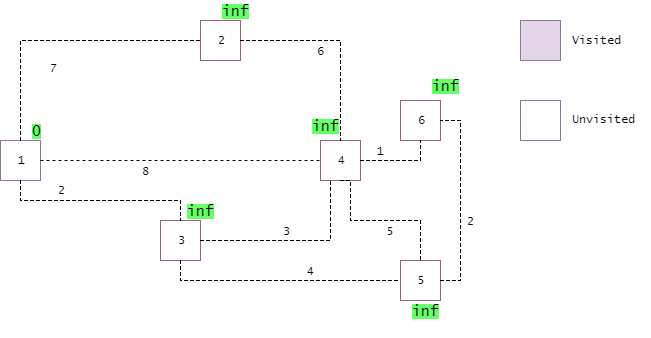
\includegraphics[width=\textwidth]{dijkstras-algorithm-example1}


\caption{After initiation of Dijkstra's algorithm}
\label{fig:dijkstras-algorithm-example1}
\end{figure}
\begin{figure}[H]
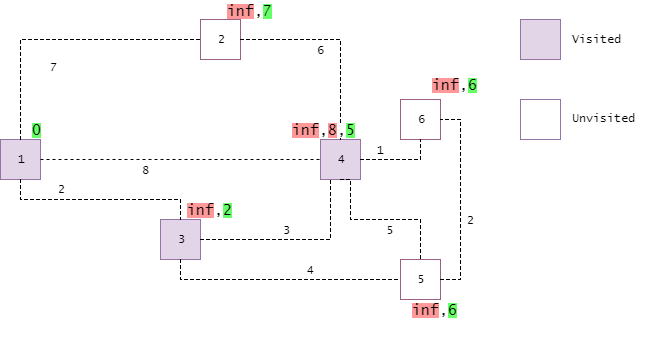
\includegraphics[width=\textwidth]{dijkstras-algorithm-example2}

\caption{After three nodes have been visited with Dijkstra's algorithm}
\label{fig:dijkstras-algorithm-example2}
\end{figure}

This algorithm will be used in a function:
\begin{description}
\item[dijkstras(graph, startNode, endNode)] - That takes graph, startNode and endNode and returns an array with the shortest path from startNode to destNode. 

\item [Algorithm description:]
\item[algorithm dijkstras(graph, startNode, endNode)]
\item[]
\begin{lstlisting}[language=Pascal]
for each node in graph
 	set dist[node] to infinity 
 	set path[node] to undefined 
end for
set dist[startNode] to 0 
set unvisitedNodes to nodes in graph
while unvisitedNodes is not empty or endNode is not in unvisitedNodes do
 	set current to node where dist[node] is smallest and node is in unvisitedNodes
 	remove current from unvisitedNodes
  	for each neighbor of current where neighbor is in unvisited do
    		set temp to dist[current] + weight of edge in graph, where edge is from current to neighbor
 		if temp is smaller than dist[neighbor] then
 			set dist[neighbor] to temp
 			set path[neighbor] to path[current] + current
 		end if
 	end for
end while
return path[endNode]
\end{lstlisting}
\end{description}
\subsection{Environment}
We will implement the algorithms using Atom \cite{atom}, a text editor, and compile and run our tests and our code with Node.js \cite{nodejs}. Tail call optimization is not available in Node.js, see \ref{sec:js-fp}. To manage our dependencies we are using npm \cite{npm}. For automation we are using Grunt \cite{grunt}. Mention github and google docs?

Since node.js does not support ES6-modules we are using babel to transpile our ES6-modules to node-modules that are supported. We are doing this since we have prior experience with ES6 modules and not with node-modules. Since node.js support almost everything else in ES6 we will only be transpiling the modules, leaving our code in an ES6 standard.

To measure memory and run time we are using node.js process, that is a global and therefore always available within node.js applications \cite{nodejs}. We are using the following functions:
\begin{description}
\item [process.hrtime(time)] - Returns the current high resolution time in a [seconds, nanoseconds] tuple Array. If the optional time-parameter, an earlier hrtime, is used, it will return the difference between that time and the current time. 
\item [process.memoryUsage()] - Returns an object describing the memory usage of the Node.js process measured in bytes.
\end{description}
\subsection{Testing}
Our code will be tested through code reviews and unit testing.
\subsubsection{Code reviews}
We will review each other's implementations and our implementations will also be reviewed by a third party. The reviews should help us to find bugs and also to confirm that we have used FP or OOP methods according to our guidelines, see \ref{sec:paradigm-guidelines}.
\subsubsection{Unit testing}
Unit testing will be done using the JavaScript libraries Mocha \cite{mocha} for writing tests, Chai \cite{chai} for evaluating expressions, and Karma \cite{karma} for automated tests.

Our implementations will have to pass the tests in appendix~\ref{appendix:test-cases} to be accepted as done.
\subsection{Implementation}
We will proceed from a template with the following structure:

\begin{lstlisting}[language=Pascal, deletekeywords={function, and}, numbers=none]
|---dist
|   \---<Files generated from babel>
|---src
|   |---js
|        |---<function and class files>
|   \---index.js
|---es6-test
|   \---<Test files>
|---test
|   \---<Test files generated from babel>
| Gruntfile.js
| package.json
\end{lstlisting}

\begin{description}
\item[] To run tests use the command:
\item[npm test] - Will transpile the test files in the es6-test-folder, place the generated files in the test-folder and run the tests.
\item[] To run the algorithm use the command:
\item[npm start] - Will transpile the JavaScript-files in src-folder, place the generated files in the dist-folder and run index.js in the dist-folder.
\end{description}

For an implementation of an algorithm to be considered done the following has to be implemented and provided:
\begin{itemize}
\item Tests for the algorithm that are defined in appendix~\ref{appendix:test-cases} placed in (projectName)/es6-test
\item A complete implementation of the algorithm that has passed the tests placed in (projectName)/src/js
\item A measurement implementation that must run the algorithm and measure time and memory usage using node.js process. The implementation must have a function for creating randomized data of a certain size according to table~\ref{tab:measurements} 
\item A timelog describing how long the implementation took. 
\end{itemize}
\subsection{Measurements}
We will measure runtime, memory usage, code length and the development time of each implementation. The measurements are done on the algorithms described in this chapter and the algorithms will run on randomized data, described in table~\ref{tab:measurements}. We are not measuring the initiation of the randomized data, except for the tree search algorithms that include an insert-function. The algorithms are measured with three different sizes of data, described in table~\ref{tab:measurements} to get more accurate results. We have chosen measurement sizes such as to avoid exceeding the call stack limit for our functional implementations.

\begin{table}[H]
\begin{tabular}{ | l p{10cm} | }
\hline
Algorithm & Binary search tree algorithms \\
Description & Should measure insert(), inOrderTraversal() and findNode(), where findNode() is run three times with a random value between 1 and 10 * n as parameter. \\
Measurement data & A binary tree with n nodes filled with randomised values between 1 and 10 * n. \\ 
Measurement sizes & n = 1000, n = 5000 and n = 10000. \\
\hline
Algorithm & Shellsort algorithm \\
Description & Should measure the shellsort-function.\\
Measurement data & An array of length n filled with randomised values between 1 and 2 * n \\ 
Measurement sizes & n = 1000, n = 3000 and n = 6000. \\
\hline
Algorithm & Tower of Hanoi algorithm \\
Description & Should measure the hanoi-algorithm where a tower is moved from one peg to another. \\
Measurement data & A tower of n disks. \\ 
Measurement sizes & n = 10, n = 20 and n = 25. \\
\hline
Algorithm & Dijkstra's algorithm \\
Description & Should measure Dijkstra's algorithm from the first node in the randomised graph to the last node in the randomised graph.\\
Measurement data & A graph with n nodes where each node is connected to the last two nodes, if those nodes exist. The edges between the nodes should be of a randomised weight between 1 and 100.\\ 
Measurement sizes & n = 10, n = 15 and n = 20. \\
\hline
\end{tabular}
\caption{Table describing measurements to be implemented}
\label{tab:measurements}
\end{table}
\subsubsection{Guidelines for implementing in the different paradigms}
\label{sec:paradigm-guidelines}
Functional programming guidelines:
\begin{itemize}
\item Do not use classes
\item Treat functions as variables
\item Compose functions to build programs
\item Use already provided pure functions when possible
\item Write pure functions
\item Do not change variables
\item Use recursion instead of iteration
\end{itemize}

Object-Oriented Programming guidelines:
\begin{itemize}
\item Use classes and objects to build programs
\item Use inheritance when possible
\item Use encapsulation
\item Each class should have only one job
\item Prefer iteration over recursion
\end{itemize}

\section{Result}
Our implementations have been reviewed by each other and also by Emil Folino that is a lecturer at BTH. The reviews worked well, but a few bugs still slipped through and had to be fixed. They were found when we noticed some strange results that we could not explain. The tests for Dijkstra's algorithm were not good enough for the functional implementation, so some manual testing had to be done.

Should we add our code here? Or should we add the code as appendices? Or should we link to github? Should we have a link to github somewhere anyway or is that not necessary?
\subsubsection{Development time and lines of code}
The total results for the development time were:
\begin{description}
\item[Kim OOP] - 20 hours and 32 minutes.
\item[Kim FP] - 18 hours and 20 minutes.
\item[Tord OOP] - 24 hours and 8 minutes.
\item[Tord FP] - 26 hours and 13 minutes.
\end{description}

Kim spent less time on the functional implementations in total, while Tord spent less time on the object-oriented implementations. For Kim she had to spend more time on the OOP solution when implementing the recursive algorithms and vice versa. Tord's results are following this pattern for the tree search algorithms and the shellsort algorithm implementations. However, he spent significantly less time on the OOP tower of hanoi algorithm than the FP implementation, and spent about as much time for both dijkstra's algorithm implementations.

\begin{figure}[H]
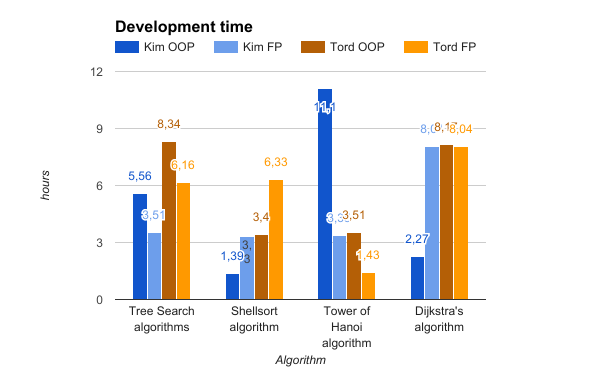
\includegraphics[width=\textwidth]{development-time-graph}

\caption{Development time for our implementations}
\label{fig:development-time-graph}
\end{figure}

The total results for the lines of code were:
\begin{description}
\item[Kim OOP] - 930 lines of code.
\item[Kim FP] - 618 lines of code.
\item[Tord OOP] - 706 lines of code.
\item[Tord FP] - 530 lines of code.
\end{description}

For both Kim and Tord the functional implementations had less code in total and individually for all implementations except for shellsort. Here both OOP implementations had the least code. We can see for Kim's tower of hanoi algorithm that there is a large difference in code length between the OOP and the FP implementations.

\begin{figure}[H]
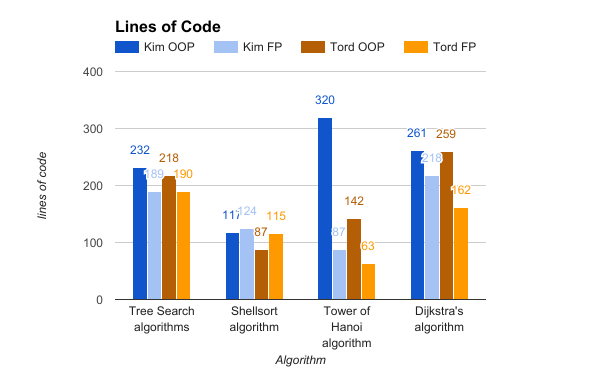
\includegraphics[width=\textwidth]{lines-of-code-graph}

\caption{Lines of code in our implementations}
\label{fig:lines-of-code-graph}
\end{figure}
\subsubsection{Search Tree Algorithms}
We can see that for Kim the functional implementation has a better runtime, but still uses a lot more memory than the object-oriented implementation. Tord's object-oriented implementation performs a lot better than his functional, both for memory usage and runtime. Tord's functional implementation is a lot slower and uses a lot more memory than all the other implementations.

\begin{figure}[H]
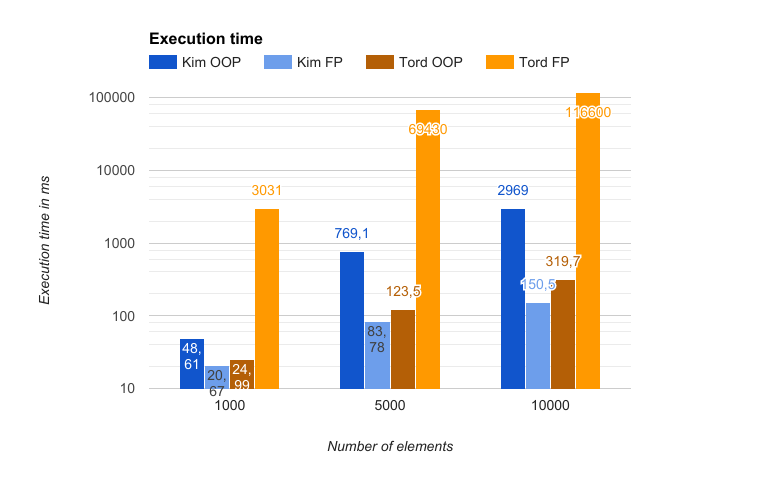
\includegraphics[width=\textwidth]{binary-tree-runtime}

\caption{Runtime for tree search implementations.}
\label{fig:binary-tree-runtime}
\end{figure}

\begin{figure}[H]
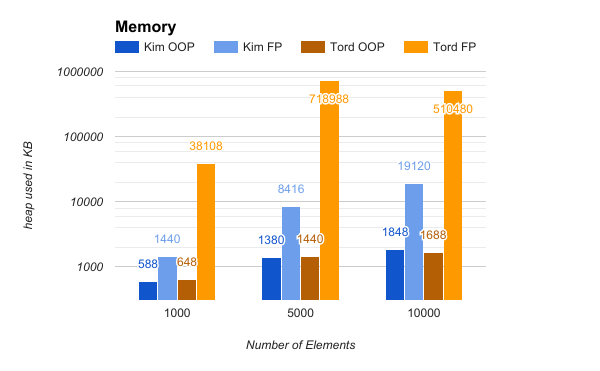
\includegraphics[width=\textwidth]{binary-tree-memory}

\caption{Memory usage for tree search implementations.}
\label{fig:binary-tree-memory}
\end{figure}
\subsubsection{Shellsort}
For shellsort Kim's and Tord's results are following the same trend. Both of their OOP implementations performed a lot better with faster runtimes and lower memory usage. We can also see that Kim's functional implementations is slower than Tord's, while Tord's is using more memory.

\begin{figure}[H]
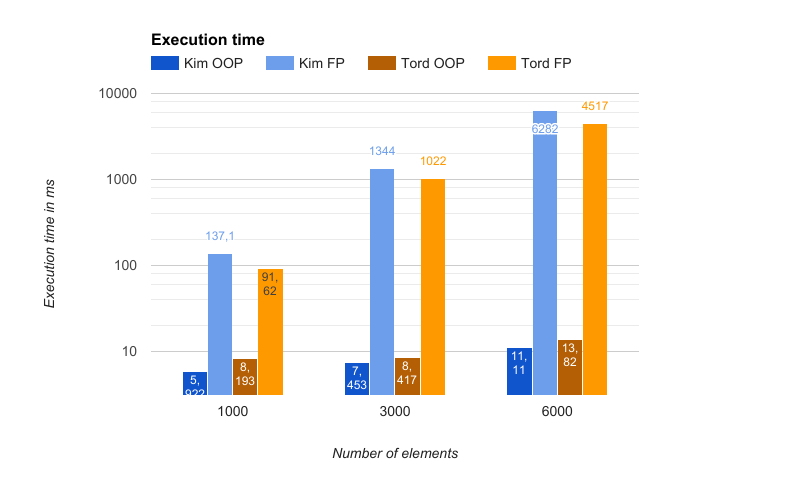
\includegraphics[width=\textwidth]{shellsort-runtime}

\caption{Runtime for shellsort implementations.}
\label{fig:shellsort-runtime}
\end{figure}

\begin{figure}[H]
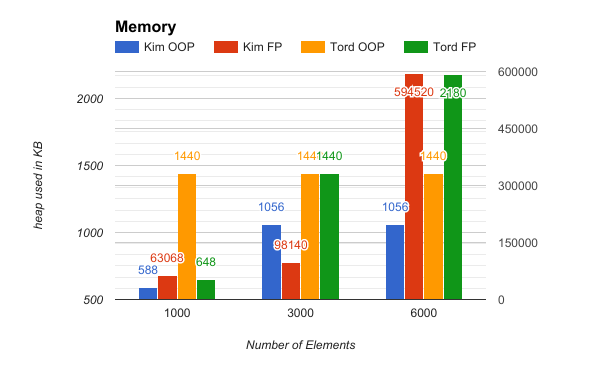
\includegraphics[width=\textwidth]{shellsort-memory}

\caption{Memory usage for shellsort implementations.}
\label{fig:shellsort-memory}
\end{figure}
\subsubsection{Tower of Hanoi}
For the Tower of Hanoi-implementations Tord's OOP implementation could not handle 25 discs because it ran out of memory. His FP implementation was faster than his OOP implementations for small tower sizes, but was the slowest of all implementations for larger. Kim's functional implementation was both faster and used less memory than her object-oriented implementation. However, there was not as big of a difference in performance between the two compared to results for other implementations.
 
\begin{figure}[H]
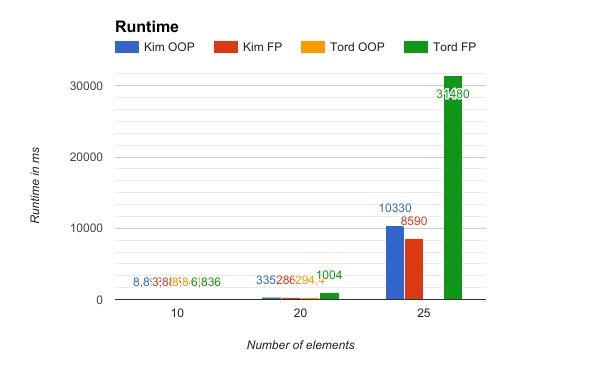
\includegraphics[width=\textwidth]{hanoi-runtime}

\caption{Runtime for hanoi implementations.}
\label{fig:hanoi-runtime}
\end{figure}

\begin{figure}[H]
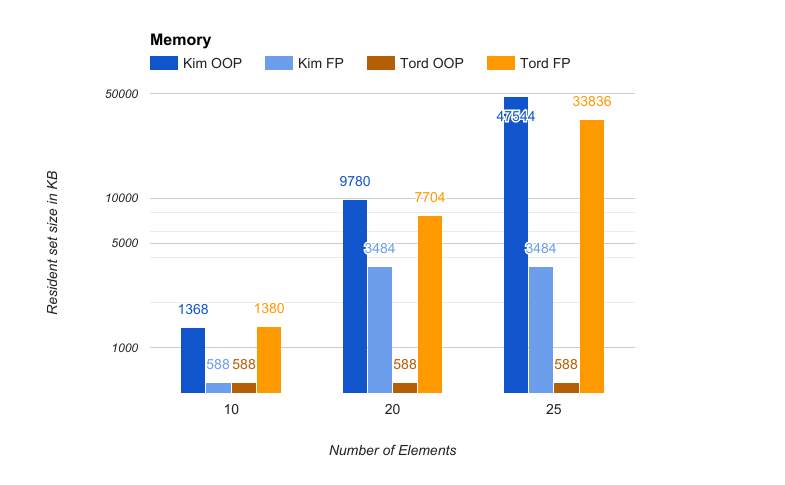
\includegraphics[width=\textwidth]{hanoi-memory}

\caption{Memory usage for hanoi implementations.}
\label{fig:hanoi-memory}
\end{figure}
\subsubsection{Dijkstra's algorithm}
Both Kim's and Tord's OOP implementations performed better than their FP implementations for Dijkstra's algorithm. Kim's FP implementation was a lot slower than all the others, while Tord's FP implementation only performed slightly worse than the OOP implementations.

\begin{figure}[H]
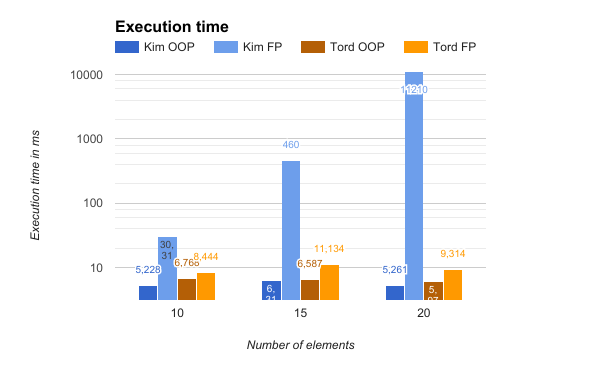
\includegraphics[width=\textwidth]{dijkstras-runtime}

\caption{Runtime usage for Dijkstra's algorithm implementations.}
\label{fig:dijkstras-runtime}
\end{figure}

\begin{figure}[H]
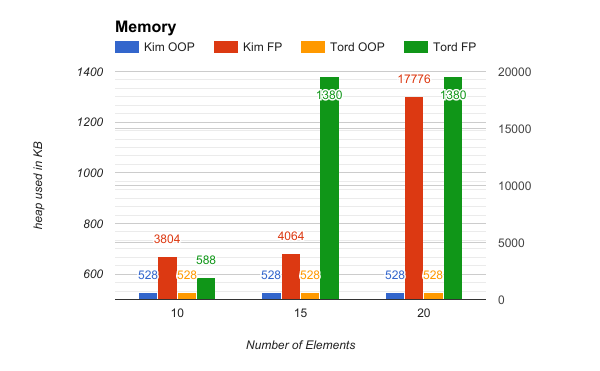
\includegraphics[width=\textwidth]{dijkstras-memory}

\caption{Memory usage for Dijkstra's algorithm implementations.}
\label{fig:dijkstras-memory}
\end{figure}

\section{Analysis}
Mostly the implementations are faster when implemented in their expected way. For example the tree search algorithms are faster recursively and the shellsort algorithm is faster iteratively. This is also clear when looking at the development time where the results suggest that we spent more time when implementing, for example, shellsort recursively or the tower of hanoi iteratively. 

We expected the development time to be shorter for the object-oriented implementations, since we both have prior experience with it and since we have nearly no prior experience with functional programming. The results show that this was not necessarily so. Neither of the paradigms seem faster to implement, however the functional paradigm might have a slight upper hand since we both had no prior experience with it. Tord's results are partly deviant from the earlier statement that we spent less or more time implementing certain algorithms depending on if it's more suited for recursion or iteration. This is clear when looking at the results for the tower of hanoi algorithm and Dijkstra's algorithm. This can be explained by that he had some trouble with tower of hanoi and used the internet for help and also that he had to rewrite and complement both of the Dijkstra's algorithms.

Over all the functional solutions had less lines of code in total and individually, except for both of our shellsort implementations. However, shellsort is a short algorithm where neither of us could add a lot of classes or methods. We both felt that this does not mean that the code is easier to read or faster to write. Rather that we simply did not implement classes with methods for the functional implementations. We both found that the lack of classes made the code messier to implement which is apparent when looking at our development time results.

For the runtime results we did expect the object-oriented implementations to be faster than the functional implementations based on \cite{hasmadole} and our research about JavaScript, see section~\ref{sec:javascript}. Overall the functional implementations performed worse than the object-oriented implementations, even though it performed better for the recursive algorithms. We both implemented very slow implementations when using functional approaches, compared to when we implemented slow implementations according to OOP. This could however be because of JavaScript. Since JavaScript does not support immutable variables we have instead treated variables as immutable by copying. This seems to take a lot of time and also use a lot of memory because of JavaScript's garbage collection. When looking at our shellsort implementations we can see that if we try to remove some of our copying our runtimes decrease a lot. Optimizing functional solutions is an option, but that would take time and would have to be considered when developing functional JavaScript. Perhaps using one of the functional libraries available would solve this problem.

Since we only had two different test groups with one person in each, it was a bit hard to analyze our results when algorithms were hard to compare. For example when an algorithm was much slower than all the others. This might not be because of the paradigm itself, but rather because the programmer has made a mistake. However, it can still give us some results as to if it is easier to make mistakes in one paradigm, but that would only be valid for that particular language. We think that it would be possible to draw more conclusions if there were more test subjects taking part in this experiment.

\section{Conclusion}
Overall we both appreciated trying out functional programming, but we don't think that we will use pure functional programming or functional languages in the future if we don't have to. We will however use a lot of the approaches that we have been using in this experiment. In our experience we found that we had less bugs when avoiding side effects and the functions were modular and easy to combine. We also liked using classes since there was a layer of abstraction on top of JavaScript's native types. We think that combining the two and using recursion or iteration when it fits best would benefit both the performance, development time and code readability. 

Based on our results different paradigms are good for different things and one is not clearly better than the other. According to our research most languages perform well, and there are also a lot of multiparadigm languages out there. Based on our results it is best to use a combination of them, especially since functional programming and object-oriented programming are not opposites. To us it makes a lot of sense that a lot of the object-oriented languages, that are based on the imperative paradigm, are starting to implement support for functional approaches. 

\section{Future Work}
In this experiment we have implemented the algorithms ourselves and compared our own work. It would be interesting to see a similar experiment with multiple test subjects that are not involved in the thesis work. 

A lot of our sources argue that functional programming should be really good for handling data concurrently. Therefore an experiment to compare different paradigms from both a performance, development and maintainability perspective would be interesting. 

We also did these implementations in JavaScript. It would be interesting to see this kind of comparison in another language that better support full functional or full OOP approaches. Perhaps comparing other paradigms and combined paradigms as well.

\bibliographystyle{IEEEtran}
\bibliography{IEEEabrv,references}
\appendix
\section{Appendix}
\label{appendix:test-cases}
\subsection{Test cases}
\begin{table}[H]
\begin{tabular}{ | l p{10cm} | }
\hline
ID & T1 \\
Algorithm & Binary search tree algorithms \\
Function & insert(comparable, rootNode) \\
Description & Inserted items should be added at the correct place in the tree. If number already exists in the binary search tree, it should not be inserted. \\
Preconditions & See figure~\ref{fig:input-tree} \\
\hline
ID & T1.1 \\
Input & 9, node(13) \\
Expected values & FP: None, OOP: See figure~\ref{fig:input-tree} \\
Expected output & FP: See figure~\ref{fig:input-tree}, OOP: false \\
\hline
ID & T1.2 \\
Input & 8, node(13) \\
Expected values & FP: None, OOP: See figure~\ref{fig:output-tree-8} \\
Expected output & FP: See figure~\ref{fig:output-tree-8}, OOP: true \\
\hline
ID & T1.3 \\
Input & 1, node(13) \\
Expected values & FP: None, OOP: See figure~\ref{fig:output-tree-1} \\
Expected output & FP: See figure~\ref{fig:output-tree-1}, OOP: true \\
\hline
ID & T1.2 \\
Input & 33, node(13) \\
Expected values & FP: None, OOP: See figure~\ref{fig:output-tree-33} \\
Expected output & FP: See figure~\ref{fig:output-tree-33}, OOP: true \\
\hline
\end{tabular}
\caption{Binary search tree algorithms insert tests}
\label{tab:insert-tests}
\end{table}

\begin{table}[H]
\begin{tabular}{ | l p{10cm} | }
\hline
ID & T2 \\
Algorithm & Binary search tree algorithms \\
Function & findNode(comparable, rootNode) \\
Description & findNode should return the node containing comparable. If comparable is not in the tree undefined should be returned. \\
Preconditions & See figure~\ref{fig:input-tree} \\
\hline
ID & T2.1 \\
Input & 5, node(13) \\
Expected values & None \\
Expected output & undefined \\
\hline
ID & T2.2 \\
Input & 13, node(13) \\
Expected values & None \\
Expected output & node(13) \\
\hline
ID & T2.3 \\
Input & 2, node(13) \\
Expected values & None \\
Expected output & node(2) \\
\hline
ID & T2.4 \\
Input & 32, node(13) \\
Expected values & None \\
Expected output & node(32) \\
\hline
ID & T2.5 \\
Input & 20, node(13) \\
Expected values & None \\
Expected output & node(20) \\
\hline
\end{tabular}
\caption{Binary search tree algorithms findNode tests}
\label{tab:find-node-tests}
\end{table}

\begin{table}[H]
\begin{tabular}{ | l p{10cm} | }
\hline
ID & T3 \\
Algorithm & Binary search tree algorithms \\
Function & inOrderTraversal() \\
Description & Should return a sorted array of the elements in the tree. If the tree is it should return an empty array. \\
\hline
ID & T3.1 \\
Preconditions & See figure~\ref{fig:input-tree} \\
Input & FP: node(13), OOP: none \\
Expected values & None \\
Expected output &  [2, 3, 6, 7, 9, 13, 16, 20, 24, 32] \\
\hline
ID & T3.2 \\
Preconditions & Empty tree \\
Input & FP: none, OOP: none \\
Expected values & None \\
Expected output & [] \\
\hline
\end{tabular}
\caption{Binary search tree algorithms inOrderTraversal tests}
\label{tab:traversal-tests}
\end{table}

\begin{table}[H]
\begin{tabular}{ | l p{10cm} | }
\hline
ID & T4 \\
Algorithm & Shellsort \\
Function & shellsort(array) \\
Description & If an array of numbers is input a sorted array should be returned. If an empty array is input an empty array should be returned. \\
Preconditions & None \\
\hline
ID & T4.1 \\
Input & [] \\
Expected values & None \\
Expected output &  [] \\
\hline
ID & T4.2 \\
Input & [ 9, 8, 1, 15, 3, 4, 11, 2, 7, 6] \\
Expected values & None \\
Expected output & [ 9, 8, 1, 15, 3, 4, 11, 2, 7, 6] \\
\hline
\end{tabular}
\caption{Shellsort tests}
\label{tab:shellsort-tests}
\end{table}

\begin{table}[H]
\begin{tabular}{ | l p{10cm} | }
\hline
ID & T5 \\
Algorithm & The Tower of Hanoi \\
Function &  hanoi(tower, start, dest, aux) \\
Description & Should return start, dest and aux pegs with moved tower. If tower has zero discs it should return empty start, dest and aux. The algorithm should take \(2^n - 1\) moves.\\
Preconditions & None \\
\hline
ID & T5.1 \\
Input & tower size 8, peg1 with tower, peg3 empty, peg2 empty \\
Expected values & FP: none, OOP: nrOfMoves=255 \\
Expected output &  peg1 empty, peg2 empty, peg3 with tower \\
\hline
ID & T5.2 \\
Input & tower size 0, peg1 empty, peg3 empty, peg2 empty \\
Expected values & FP: none, OOP: nrOfMoves=0 \\
Expected output & peg1 empty, peg2 empty, peg3 empty \\
\hline
\end{tabular}
\caption{Tower of Hanoi algorithm tests}
\label{tab:tower-of-hanoi-tests}
\end{table}

\begin{table}[H]
\begin{tabular}{ | l p{10cm} | }
\hline
ID & T6 \\
Algorithm & Dijksta's algorithm \\
Function & dijkstras(graph, startNode, endNode) \\
Description & Should return the shortest path from startNode to endNode. If startNode is same as endNode it should return empty path. If graph is empty it should return empy path.\\
Preconditions & None \\
\hline
ID & T6.1 \\
Input & See figure~\ref{fig:input-graph}, node1, node6 \\
Expected values & None \\
Expected output &  See figure~\ref{fig:output-graph} \\
\hline
ID & T6.2 \\
Input & See figure~\ref{fig:input-graph}, node1, node4 \\
Expected values & None \\
Expected output &  See figure~\ref{fig:output-graph2} \\
\hline
ID & T6.3 \\
Input & See figure~\ref{fig:input-graph}, node2, node5 \\
Expected values & None \\
Expected output &  See figure~\ref{fig:output-graph3} \\
\hline
ID & T6.4 \\
Input & See figure~\ref{fig:input-graph}, node1, node1\\
Expected values & None \\
Expected output & empty path \\
\hline
ID & T6.5 \\
Input & nodes=[], edges[], noNode, noNode \\
Expected values & None \\
Expected output & empty path \\
\hline
\end{tabular}
\caption{Dijkstra's algorithm tests}
\label{tab:dijkstras-tests}
\end{table}
\subsection{Test case images}
\begin{figure}[H]
\includegraphics[width=\textwidth]{input-tree}

\caption{Input tree}
\label{fig:input-tree}
\end{figure}

\begin{figure}[H]
\includegraphics[width=\textwidth]{output-tree-8}

\caption{Output tree after inserting 8}
\label{fig:output-tree-8}
\end{figure}

\begin{figure}[H]
\includegraphics[width=\textwidth]{output-tree-1}

\caption{Output tree after inserting 1}
\label{fig:output-tree-1}
\end{figure}

\begin{figure}[H]
\includegraphics[width=\textwidth]{output-tree-33}

\caption{Output tree after inserting 33}
\label{fig:output-tree-33}
\end{figure}

\begin{figure}[H]
\includegraphics[width=\textwidth]{input-graph}

\caption{Input graph}
\label{fig:input-graph}
\end{figure}

\begin{figure}[H]
\includegraphics[width=\textwidth]{output-graph}

\caption{Output graph 1}
\label{fig:output-graph}
\end{figure}

\begin{figure}[H]
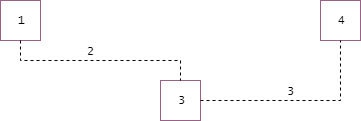
\includegraphics[width=\textwidth]{output-graph2}

\caption{Output graph 2}
\label{fig:output-graph2}
\end{figure}

\begin{figure}[H]
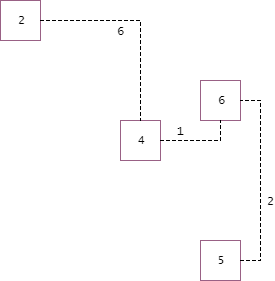
\includegraphics[width=\textwidth]{output-graph3}

\caption{Output graph 3}
\label{fig:output-graph3}
\end{figure}

\end{document}

